\documentclass[11pt]{article}
\usepackage[margin=1in]{geometry}
\usepackage{graphicx}
\usepackage{booktabs}
\usepackage{tabularx}
\usepackage{array}
\usepackage{hyperref}
\usepackage{amsmath}

\title{PCU MVP Demo Documentation}
\author{Project Team}
\date{\today}

\begin{document}
\maketitle

\section{Purpose and High-Level Idea}
The Personalized Care Unit (PCU) is a continuous, person-centered AI system for day-scale health support. The working unit is not a single isolated reading. The working unit is a personal event in time, such as meal start, post-meal glucose trajectory, exercise transition, wake window, or pre-bed window. PCU links events across multiple time scales (minute, short window, and daily pattern) and updates recommendations as the day evolves.

This MVP demonstrates PCU in a combined scenario of Type II diabetes support and social-wellness monitoring. The system continuously monitors incoming signals, detects actionable events, estimates risk, and delivers concise behavioral guidance at the moment it is useful. In this demo, outputs are decision-support messages, not diagnosis or medication dosing.

\section{System Boundary in This MVP}
This MVP is a replay-based demonstration. Historical records are played back in temporal order to verify end-to-end PCU behavior. The active boundary includes event detection, state estimation, contextual inference, knowledge retrieval, orchestration, guidance generation, safety screening, and user-facing delivery. The runtime entry point is \texttt{GET /api/pcu}.

The primary replay dataset is \texttt{CGMacros-015}. This participant file is multimodal and includes aligned fields that combine glucose-related records with additional behavioral streams. Outputs are rendered in three surfaces: chatbot view, dashboard view, and caregiver-oriented view.

\begin{figure}[t]
    \centering
    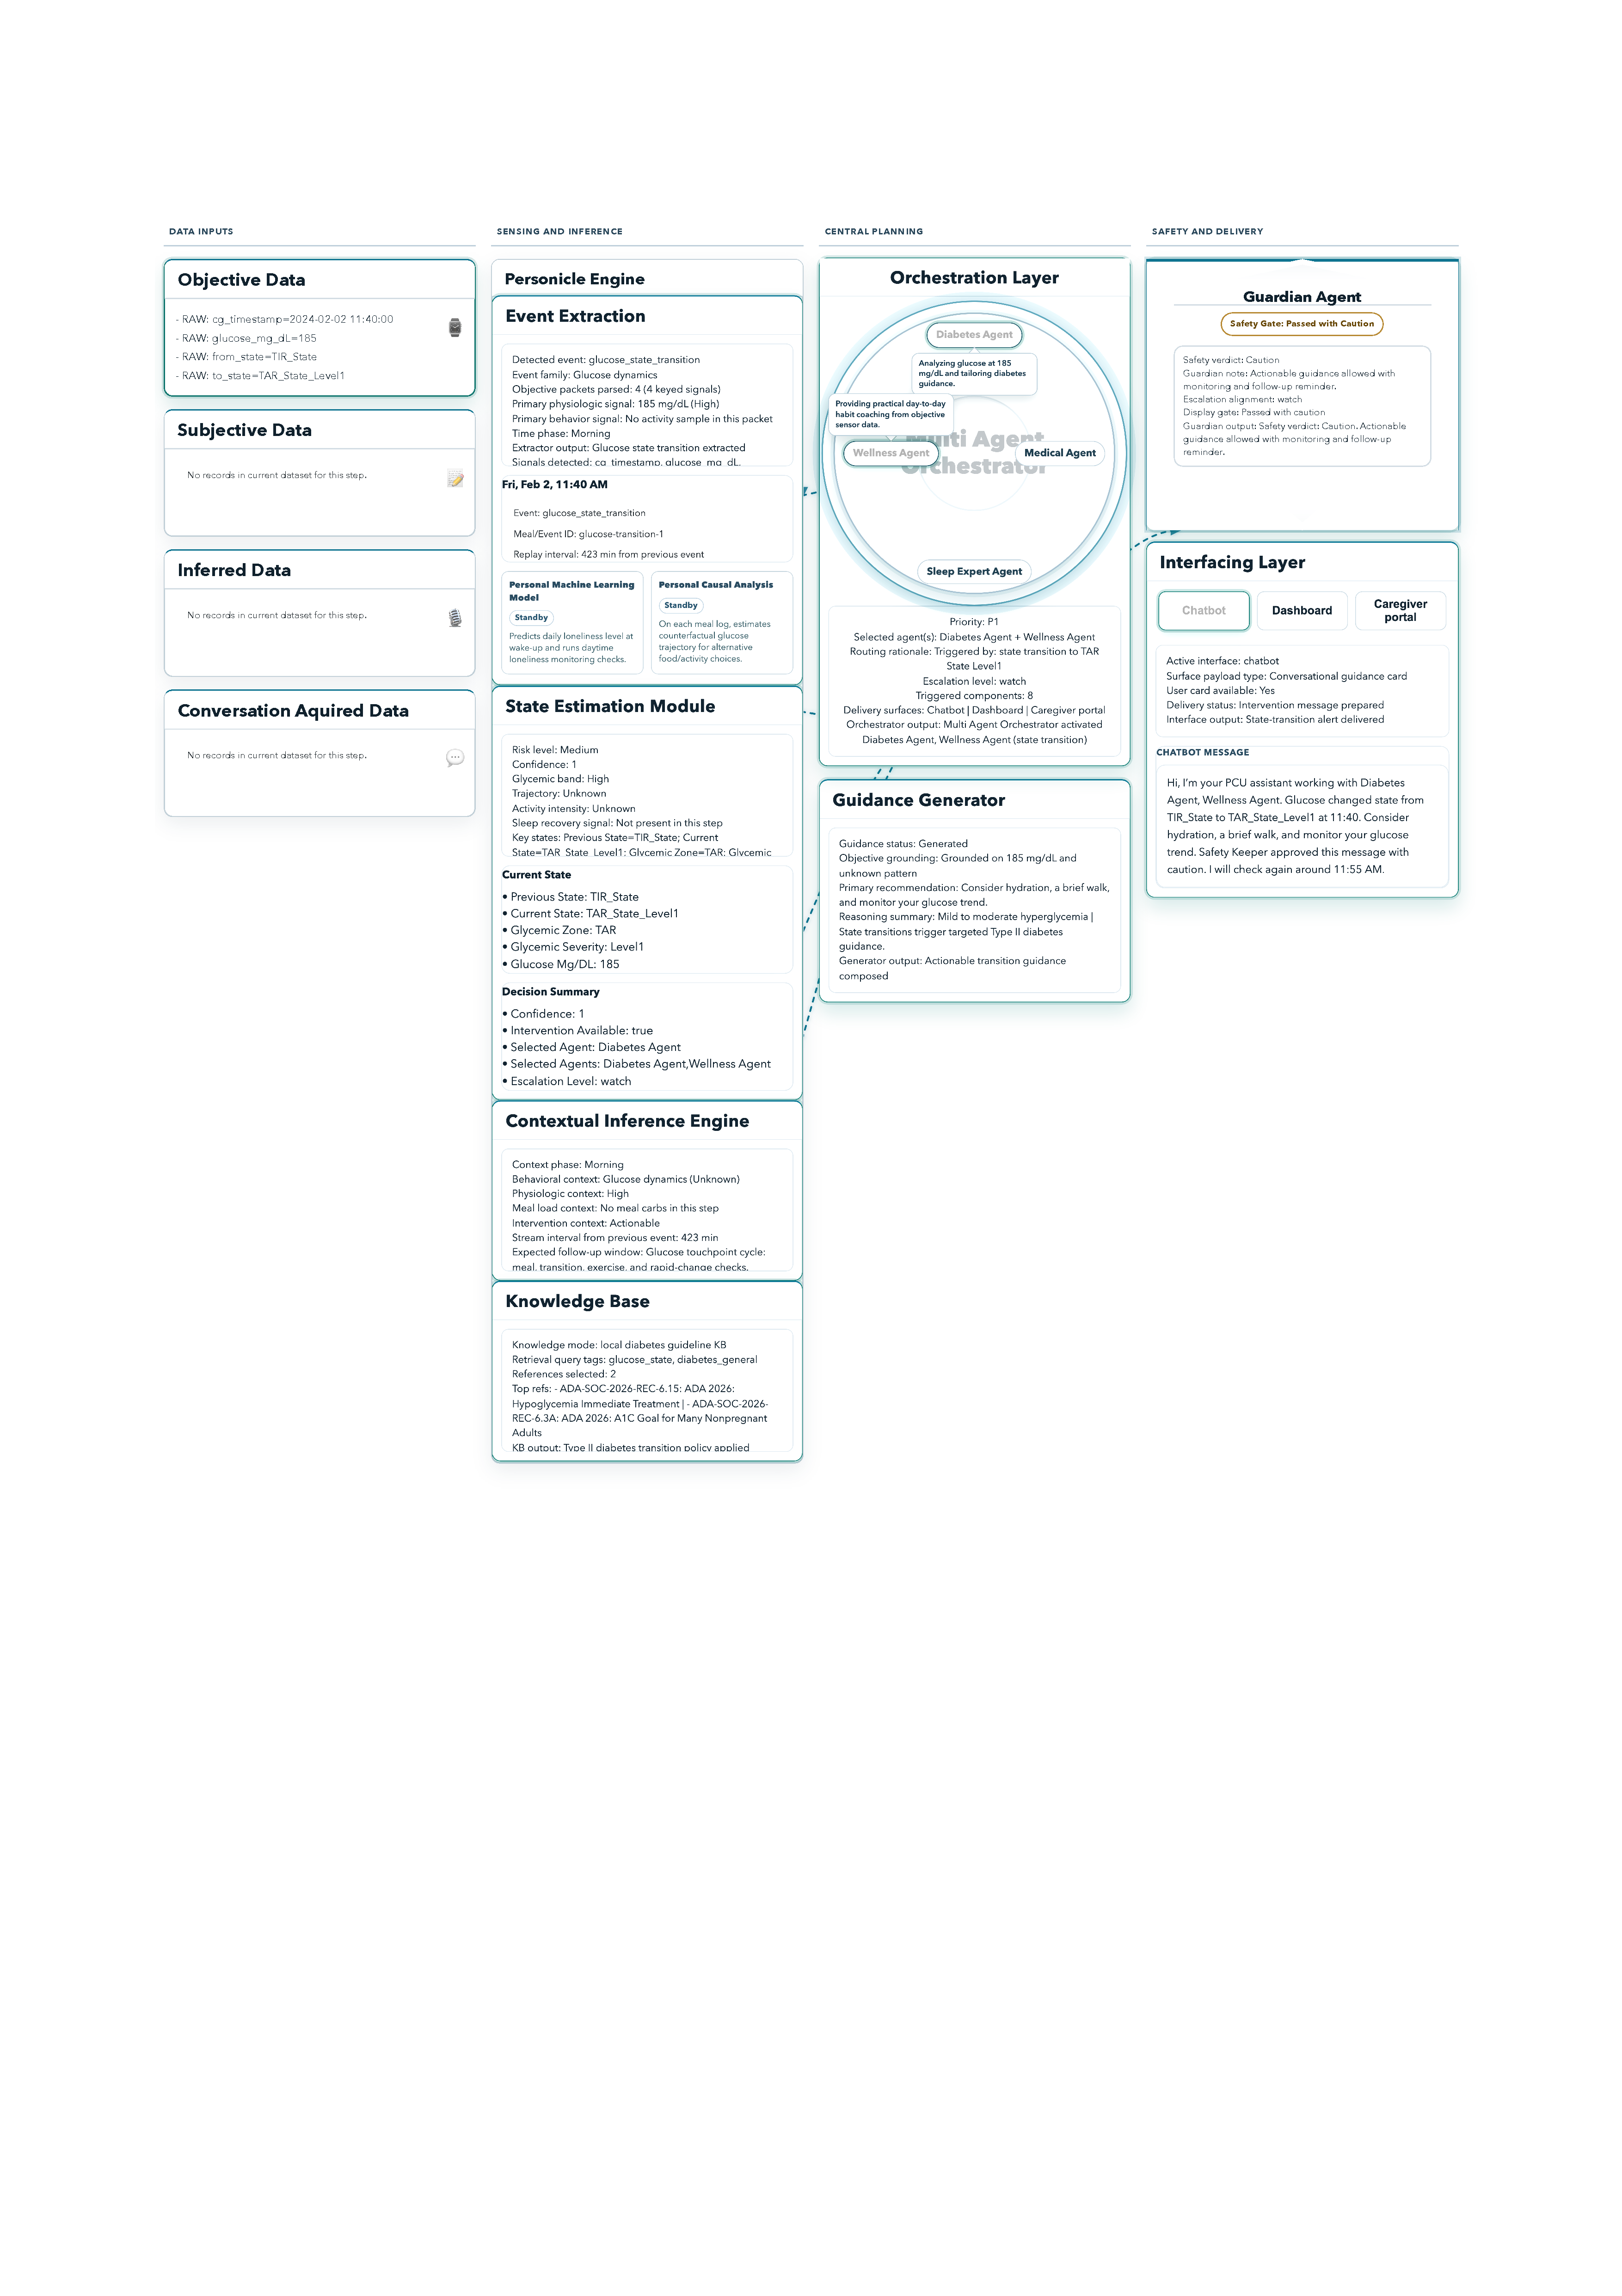
\includegraphics[width=\textwidth,page=1]{pcu_demo_playback.pdf}
    \caption{PCU MVP playback interface with active component outputs and user-facing guidance.}
    \label{fig:pcu-ui}
\end{figure}

\section{Input Model and Data Provenance}
\subsection{Input Channels}
PCU defines four channels so that multimodal expansion remains explicit even when some modalities are not populated in one run.

\begin{table}[h]
\centering
\begin{tabularx}{\textwidth}{>{\raggedright\arraybackslash}p{0.2\textwidth} >{\raggedright\arraybackslash}p{0.2\textwidth} >{\raggedright\arraybackslash}X >{\raggedright\arraybackslash}p{0.2\textwidth}}
\toprule
Channel & Source Ownership & Typical Signals & MVP Status \\
\midrule
Objective Data & User wearable and logged behavior data & CGM glucose, meal metadata, activity MET, sleep timing and sleep score & Active \\
Subjective Data & User self-report & Mood, stress, symptoms, daily reflection & Schema present; not populated in this replay \\
Inferred Data & Models derived from user history and current stream & Latent risk states and projected trajectories & Partially active via Personiclie outputs \\
Conversation Acquired Data & User-agent dialogue & Clarifications, preferences, barriers, and intent updates & Schema present; not populated in this replay \\
\bottomrule
\end{tabularx}
\caption{PCU input channels and coverage in the current MVP run.}
\label{tab:inputs}
\end{table}

\subsection{Where Inputs Come From in This Demo}
The active replay path reads \texttt{Oura/activity\_1min.csv} and \texttt{Oura/sleep\_daily.csv} under \texttt{CGMacros-015}. The activity stream contributes timestamped glucose, meal tags, carbohydrate amount, and activity intensity. The sleep stream contributes sleep duration, sleep score, and wake/bed timing indicators. The same records include provenance fields (\texttt{cg\_*} and \texttt{lon\_*}) to preserve cross-study alignment traceability in the synthetic fused dataset.

\section{Expected Deliverables to Users}
Each PCU intervention is delivered as a short structured message that answers three practical questions: what changed, why it matters now, and what action is recommended next. Deliverables include event cards for routine decisions, risk-focused alerts when thresholds are severe, and explanation traces for caregiver-facing review.

\begin{table}[h]
\centering
\begin{tabularx}{\textwidth}{>{\raggedright\arraybackslash}p{0.23\textwidth} >{\raggedright\arraybackslash}X >{\raggedright\arraybackslash}p{0.25\textwidth}}
\toprule
Deliverable Type & Content & Delivery Surface \\
\midrule
Event Card & Event title, state change summary, rationale, and next action & Chatbot, dashboard \\
Risk Alert & Escalated wording for severe hypo/hyperglycemic conditions and urgent follow-up & Chatbot, caregiver portal \\
Routine Nudge & Meal-start, post-meal, exercise-recovery, and pre-bed actions with timing & Chatbot, dashboard \\
Traceable Context & Activated agents, policy references, and state snapshot for audit & Caregiver portal, technical review \\
\bottomrule
\end{tabularx}
\caption{User-facing deliverables produced by the MVP pipeline.}
\label{tab:deliverables}
\end{table}

\section{Functional Description of PCU Components}
\subsection{Personiclie Super-Block (Sensing and Inference Column)}
In this report, Personiclie is defined as a \textbf{super-block} that contains the core sensing-and-inference components. Specifically, the Personiclie block contains event extraction, state estimation, contextual inference, and the personal knowledge layer. These modules are internal components of Personiclie, not parallel peers.

Operationally, Personiclie converts raw multimodal streams into personal event memory and decision-ready personal context. In this MVP, it produces both physiological event signals and personal model signals, including meal-level counterfactual projections and loneliness-risk estimates.

\subsubsection{Event Extraction Module}
This internal module detects temporal events from raw streams, including meal start, post-meal checkpoints, glucose transitions, rapid rise/fall, exercise start/end, wake events, and pre-bed reminders. Its function is to identify \emph{when} an intervention opportunity or risk transition occurs.

\subsubsection{State Estimation Module}
This internal module converts each event window into normalized state variables. For meal windows, it computes baseline glucose, post-meal peak, delta from baseline, and confidence of window completeness. For exercise and sleep windows, it computes recovery-relevant state descriptors. These variables are the numerical basis for subsequent decision logic.

\subsubsection{Contextual Inference Engine}
This internal module maps state variables to interpretable situation labels, including after-meal trajectory, during exercise, post-exercise recovery, wake-up context, and pre-bed context. This step prevents context-free recommendations and makes action selection time-aware.

\subsubsection{Personal Knowledge Layer}
This internal layer is derived from user-specific history and recurring response patterns. It stores person-level response memory and supports personalized interpretation of current events.

\subsection{Population Knowledge Base (outside Personiclie)}
This layer provides policy constraints external to Personiclie. In this MVP, population policy grounding is provided by curated ADA Standards of Care in Diabetes-2026 entries. Recommendations are generated by combining Personiclie outputs with this external policy layer.

\subsection{Orchestration Layer (outside Personiclie)}
This layer selects and coordinates specialist agents, including Diabetes, Sleep Expert, Wellness, and Medical roles. In the future design, this layer is intended to be an LLM-agent coordinator with explicit tool and policy interfaces. In this MVP, orchestration is implemented with transparent rule-based routing so trigger-to-action logic remains auditable.

\subsection{Guidance Generator (outside Personiclie)}
This layer converts selected action intents into concise user language with explicit timing. In future realization, this can be implemented by a dedicated LLM agent with stronger personalization and language adaptation. In the current demo, generation is template-constrained and behavior-focused to keep outputs safe and consistent.

\subsection{Guardian Agent (outside Personiclie)}
This layer is the final safety gate before delivery. In the target architecture, specialist components are LLM agents with explicit safety governance. In this MVP, these agents are represented by rule-based placeholders, and the guardian applies severity-aware wording and escalation framing when thresholds indicate high risk.

\subsection{Interfacing Layer (outside Personiclie)}
This layer presents the final decision payload across chatbot, dashboard, and caregiver views. It keeps delivery independent from core reasoning logic and allows the same recommendation to be rendered for different user roles.

\section{Overall PCU Workflow}
PCU operates as a closed loop. First, multimodal user data are aligned by timestamp and passed into the Personiclie super-block. Inside Personiclie, event extraction, state estimation, contextual inference, and personal knowledge update are executed to produce decision-ready personal context. Next, orchestration chooses specialist reasoning paths and combines personal and population knowledge. Then, the guidance module constructs user instructions, and the guardian verifies safety framing. Finally, the interfacing layer delivers the recommendation and the system continues monitoring, so each delivered intervention is immediately followed by new observation and potential adjustment.

The loop can be summarized compactly as:
\[
\begin{aligned}
\text{Multimodal User Streams}
&\rightarrow \text{Personiclie Super-Block} \\
&\hspace{1.2em}(\text{Event + State + Context + Personal Knowledge}) \\
&\rightarrow \text{Orchestration + Knowledge Retrieval} \\
&\rightarrow \text{Guidance Generation + Safety Gate} \\
&\rightarrow \text{User Delivery + Continued Monitoring}
\end{aligned}
\]

\subsection{Concrete Demo Walkthrough}
In this demo, the day begins with wake detection and a recovery-aware morning plan. At meal start, the system evaluates baseline glucose and meal composition and emits a proactive meal-start action. Around 45 minutes later, it checks post-meal trajectory and, if risk is elevated, sends a correction step such as short movement and timed recheck. During and after exercise, it evaluates glucose safety and recovery state. In the evening, it evaluates dinner response and finally delivers pre-bed guidance to stabilize overnight recovery. This sequence demonstrates continuous intervention rather than one-shot recommendation.

\section{Example One-Day Workflow}
Table~\ref{tab:workflow} summarizes one representative day in compact form.

\begin{table}[h]
\centering
\small
\setlength{\tabcolsep}{4pt}
\begin{tabularx}{\textwidth}{>{\raggedright\arraybackslash}p{0.12\textwidth} >{\raggedright\arraybackslash}p{0.26\textwidth} >{\raggedright\arraybackslash}X}
\toprule
Stage & System Operation (Input and Processing) & User Deliverable \\
\midrule
Morning wake & Detect wake context from sleep timing and prior sleep score; update morning recovery state and run personal loneliness predictor. & Morning check-in with day setup guidance for meal load, movement, and social stabilization. \\
Breakfast & Read meal type, carbs, baseline glucose, and current activity; create meal-start risk profile and candidate intervention plan. & Meal-start card with immediate low-risk action and expected effect. \\
Post-meal check & Evaluate glucose at approximately +45 minutes and delta from baseline; route to diabetes or medical handling if threshold is severe. & Corrective nudge with explicit recheck timing. \\
Exercise window & Detect exercise start/end from MET trajectory and compare glucose before, during, and after activity. & Exercise safety and recovery guidance. \\
Afternoon monitor & Re-evaluate day-level social-wellness risk from ongoing activity and recovery features. & Social well-being prompt when moderate or high risk is detected. \\
Dinner and evening & Repeat meal-response analysis in evening context and evaluate carry-over risk into sleep period. & Dinner-specific adjustment guidance. \\
Pre-bed & Trigger reminder before inferred bedtime and apply sleep-focused policy constraints. & Pre-bed routine recommendation to improve overnight stability. \\
\bottomrule
\end{tabularx}
\caption{One-day PCU workflow with processing logic and delivered outputs.}
\label{tab:workflow}
\end{table}

\section{Input, Processing, and Deliverable Contract}
For each timeline event, the MVP exposes a structured contract from intake to output. The input trace records raw received fields and grouped channels. The processing trace records activated components, state snapshot, decision snapshot, and selected agents. The deliverable trace records \texttt{title}, \texttt{what\_happened}, \texttt{why}, and \texttt{try\_next\_time}. This contract supports technical audit and makes it clear where rule-based placeholders are currently used.

\section{MVP Safety and Scope}
This MVP is a behavior-support and decision-support prototype. It is not a diagnostic engine and does not provide medication dosing instructions. Recommendations are designed for safe self-management prompts and escalation framing when severe thresholds are detected.

\appendix
\section{Data Used in This MVP Demo}
\subsection{Synthetic Dataset Definition}
This demo uses a synthetic multimodal fusion dataset described in \texttt{SYNTHETIC\_DATASET\_INTRODUCTION.md}. The synthetic data are not generated from random simulation. They are produced by cross-study alignment between CGMacros participant-day records and behaviorally matched days from a loneliness dataset, followed by timestamp warping.

\subsection{How the Synthetic Data Are Constructed}
Construction follows two steps. First, day-level matching is computed from activity profiles using cosine similarity. Second, minute-level dynamic time warping (DTW) maps source timestamps onto the CG timeline. The result is a fused participant-day view with explicit provenance fields that retain both synthetic target identity and source identity.

\subsection{Core Provenance Fields}
Rows contain alignment and provenance fields such as \texttt{cg\_participant}, \texttt{cg\_date}, \texttt{cg\_timestamp}, \texttt{lon\_participant}, \texttt{lon\_date}, and \texttt{lon\_timestamp}. These fields are required for correct interpretation. They indicate alignment relationships, not naturally co-collected same-person measurements.

\subsection{Observed Coverage in the Synthetic Introduction File}
\begin{table}[h]
\centering
\begin{tabularx}{\textwidth}{>{\raggedright\arraybackslash}X >{\raggedleft\arraybackslash}p{0.25\textwidth}}
\toprule
Coverage Item & Reported Value \\
\midrule
Synthetic participant folders generated & 34 \\
Matched CG participant-days & 375 \\
Unique loneliness source participants used & 31 \\
Minute-level DTW mappings & 501{,}078 \\
Mean cosine similarity of day matching & 0.8604 \\
Mean DTW cost across mapped minutes & 606.24 \\
\bottomrule
\end{tabularx}
\caption{Key synthetic dataset statistics summarized from the project introduction file.}
\label{tab:synthetic-stats}
\end{table}

\subsection{Active Files in This Replay Pipeline}
Although the synthetic export includes multiple modalities, the current MVP replay path actively consumes \texttt{Oura/activity\_1min.csv} and \texttt{Oura/sleep\_daily.csv} for event generation and state updates. Policy grounding is loaded from \texttt{mvp/backend/knowledge/diabetes\_guidelines.json}.

\section{Component Status and Placeholder Notes}
\begin{table}[h]
\centering
\begin{tabularx}{\textwidth}{>{\raggedright\arraybackslash}p{0.34\textwidth} >{\raggedright\arraybackslash}p{0.19\textwidth} >{\raggedright\arraybackslash}X}
\toprule
Component & Status in MVP & Note \\
\midrule
Personiclie super-block (sensing and inference) & Implemented, mixed granularity & Parent block containing event extraction, state estimation, contextual inference, and personal knowledge. \\
Event Extraction Module (inside Personiclie) & Implemented & Detects event triggers from multimodal streams. \\
State Estimation Module (inside Personiclie) & Implemented & Computes glucose and recovery state snapshots for each event window. \\
Contextual Inference Engine (inside Personiclie) & Implemented & Produces context labels required for policy-correct decisions. \\
Personal Knowledge Layer (inside Personiclie) & Partially implemented & Derived from user history and model signals in current replay scope. \\
Population Knowledge Base (outside Personiclie) & Implemented & Guideline-grounded entries from ADA policy file. \\
Orchestration Layer & Placeholder implementation & Rule-based routing in demo; target design is LLM-agent orchestration. \\
Guidance Generator & Placeholder implementation & Template-based generation in demo; target design is agentic language generation. \\
Guardian Agent & Placeholder implementation & Rule-based safety screening in demo; target design is policy-aware safety agent. \\
Interfacing Layer & Implemented & Stable output schema rendered in chatbot, dashboard, and caregiver views. \\
\bottomrule
\end{tabularx}
\caption{Current implementation status and planned evolution of each PCU component.}
\label{tab:status}
\end{table}

\end{document}
